% Options for packages loaded elsewhere
\PassOptionsToPackage{unicode}{hyperref}
\PassOptionsToPackage{hyphens}{url}
%
\documentclass[
  ,man,floatsintext]{apa6}
\usepackage{amsmath,amssymb}
\usepackage{iftex}
\ifPDFTeX
  \usepackage[T1]{fontenc}
  \usepackage[utf8]{inputenc}
  \usepackage{textcomp} % provide euro and other symbols
\else % if luatex or xetex
  \usepackage{unicode-math} % this also loads fontspec
  \defaultfontfeatures{Scale=MatchLowercase}
  \defaultfontfeatures[\rmfamily]{Ligatures=TeX,Scale=1}
\fi
\usepackage{lmodern}
\ifPDFTeX\else
  % xetex/luatex font selection
  \setmainfont[]{Times New Roman}
\fi
% Use upquote if available, for straight quotes in verbatim environments
\IfFileExists{upquote.sty}{\usepackage{upquote}}{}
\IfFileExists{microtype.sty}{% use microtype if available
  \usepackage[]{microtype}
  \UseMicrotypeSet[protrusion]{basicmath} % disable protrusion for tt fonts
}{}
\usepackage{xcolor}
\usepackage{graphicx}
\makeatletter
\def\maxwidth{\ifdim\Gin@nat@width>\linewidth\linewidth\else\Gin@nat@width\fi}
\def\maxheight{\ifdim\Gin@nat@height>\textheight\textheight\else\Gin@nat@height\fi}
\makeatother
% Scale images if necessary, so that they will not overflow the page
% margins by default, and it is still possible to overwrite the defaults
% using explicit options in \includegraphics[width, height, ...]{}
\setkeys{Gin}{width=\maxwidth,height=\maxheight,keepaspectratio}
% Set default figure placement to htbp
\makeatletter
\def\fps@figure{htbp}
\makeatother
\setlength{\emergencystretch}{3em} % prevent overfull lines
\providecommand{\tightlist}{%
  \setlength{\itemsep}{0pt}\setlength{\parskip}{0pt}}
\setcounter{secnumdepth}{-\maxdimen} % remove section numbering
% Make \paragraph and \subparagraph free-standing
\ifx\paragraph\undefined\else
  \let\oldparagraph\paragraph
  \renewcommand{\paragraph}[1]{\oldparagraph{#1}\mbox{}}
\fi
\ifx\subparagraph\undefined\else
  \let\oldsubparagraph\subparagraph
  \renewcommand{\subparagraph}[1]{\oldsubparagraph{#1}\mbox{}}
\fi
\newlength{\cslhangindent}
\setlength{\cslhangindent}{1.5em}
\newlength{\csllabelwidth}
\setlength{\csllabelwidth}{3em}
\newlength{\cslentryspacingunit} % times entry-spacing
\setlength{\cslentryspacingunit}{\parskip}
\newenvironment{CSLReferences}[2] % #1 hanging-ident, #2 entry spacing
 {% don't indent paragraphs
  \setlength{\parindent}{0pt}
  % turn on hanging indent if param 1 is 1
  \ifodd #1
  \let\oldpar\par
  \def\par{\hangindent=\cslhangindent\oldpar}
  \fi
  % set entry spacing
  \setlength{\parskip}{#2\cslentryspacingunit}
 }%
 {}
\usepackage{calc}
\newcommand{\CSLBlock}[1]{#1\hfill\break}
\newcommand{\CSLLeftMargin}[1]{\parbox[t]{\csllabelwidth}{#1}}
\newcommand{\CSLRightInline}[1]{\parbox[t]{\linewidth - \csllabelwidth}{#1}\break}
\newcommand{\CSLIndent}[1]{\hspace{\cslhangindent}#1}
\ifLuaTeX
\usepackage[bidi=basic]{babel}
\else
\usepackage[bidi=default]{babel}
\fi
\babelprovide[main,import]{english}
\ifPDFTeX
\else
\babelfont[english]{rm}{Times New Roman}
\fi
% get rid of language-specific shorthands (see #6817):
\let\LanguageShortHands\languageshorthands
\def\languageshorthands#1{}
% Manuscript styling
\usepackage{upgreek}
\captionsetup{font=singlespacing,justification=justified}

% Table formatting
\usepackage{longtable}
\usepackage{lscape}
% \usepackage[counterclockwise]{rotating}   % Landscape page setup for large tables
\usepackage{multirow}		% Table styling
\usepackage{tabularx}		% Control Column width
\usepackage[flushleft]{threeparttable}	% Allows for three part tables with a specified notes section
\usepackage{threeparttablex}            % Lets threeparttable work with longtable

% Create new environments so endfloat can handle them
% \newenvironment{ltable}
%   {\begin{landscape}\centering\begin{threeparttable}}
%   {\end{threeparttable}\end{landscape}}
\newenvironment{lltable}{\begin{landscape}\centering\begin{ThreePartTable}}{\end{ThreePartTable}\end{landscape}}

% Enables adjusting longtable caption width to table width
% Solution found at http://golatex.de/longtable-mit-caption-so-breit-wie-die-tabelle-t15767.html
\makeatletter
\newcommand\LastLTentrywidth{1em}
\newlength\longtablewidth
\setlength{\longtablewidth}{1in}
\newcommand{\getlongtablewidth}{\begingroup \ifcsname LT@\roman{LT@tables}\endcsname \global\longtablewidth=0pt \renewcommand{\LT@entry}[2]{\global\advance\longtablewidth by ##2\relax\gdef\LastLTentrywidth{##2}}\@nameuse{LT@\roman{LT@tables}} \fi \endgroup}

% \setlength{\parindent}{0.5in}
% \setlength{\parskip}{0pt plus 0pt minus 0pt}

% Overwrite redefinition of paragraph and subparagraph by the default LaTeX template
% See https://github.com/crsh/papaja/issues/292
\makeatletter
\renewcommand{\paragraph}{\@startsection{paragraph}{4}{\parindent}%
  {0\baselineskip \@plus 0.2ex \@minus 0.2ex}%
  {-1em}%
  {\normalfont\normalsize\bfseries\itshape\typesectitle}}

\renewcommand{\subparagraph}[1]{\@startsection{subparagraph}{5}{1em}%
  {0\baselineskip \@plus 0.2ex \@minus 0.2ex}%
  {-\z@\relax}%
  {\normalfont\normalsize\itshape\hspace{\parindent}{#1}\textit{\addperi}}{\relax}}
\makeatother

% \usepackage{etoolbox}
\makeatletter
\patchcmd{\HyOrg@maketitle}
  {\section{\normalfont\normalsize\abstractname}}
  {\section*{\normalfont\normalsize\abstractname}}
  {}{\typeout{Failed to patch abstract.}}
\patchcmd{\HyOrg@maketitle}
  {\section{\protect\normalfont{\@title}}}
  {\section*{\protect\normalfont{\@title}}}
  {}{\typeout{Failed to patch title.}}
\makeatother

\usepackage{xpatch}
\makeatletter
\xapptocmd\appendix
  {\xapptocmd\section
    {\addcontentsline{toc}{section}{\appendixname\ifoneappendix\else~\theappendix\fi\\: #1}}
    {}{\InnerPatchFailed}%
  }
{}{\PatchFailed}
\usepackage{csquotes}
\usepackage{threeparttable}
\usepackage{setspace}\singlespacing
\usepackage{dcolumn}
\usepackage{upgreek}
\setlength{\parskip}{0pt}
\raggedbottom
\ifLuaTeX
  \usepackage{selnolig}  % disable illegal ligatures
\fi
\IfFileExists{bookmark.sty}{\usepackage{bookmark}}{\usepackage{hyperref}}
\IfFileExists{xurl.sty}{\usepackage{xurl}}{} % add URL line breaks if available
\urlstyle{same}
\hypersetup{
  pdftitle={Selective Attention Adapts to Blockwise but Not Location-Based Proportion-Congruence with Trial-Unique Stimuli},
  pdfauthor={Jack Dolgin1 \& Tobias Egner2},
  pdflang={en-EN},
  hidelinks,
  pdfcreator={LaTeX via pandoc}}

\title{Selective Attention Adapts to Blockwise but Not Location-Based Proportion-Congruence with Trial-Unique Stimuli}
\author{Jack Dolgin\textsuperscript{1} \& Tobias Egner\textsuperscript{2}}
\date{}


\shorttitle{Attention Adapts to Blocks, but Not Locations}

\authornote{

Correspondence concerning this article should be addressed to Jack Dolgin, Somers Family Hall 1125, 1 Brookings Drive, St.~Louis, MO 63105. E-mail: \href{mailto:jdolgin@wustl.edu}{\nolinkurl{jdolgin@wustl.edu}}

}

\affiliation{\vspace{0.5cm}\textsuperscript{1} Washington University in St.~Louis\\\textsuperscript{2} Duke University}

\begin{document}
\maketitle

\hypertarget{introduction}{%
\section{Introduction}\label{introduction}}

Cognitive control denotes our ability to use temporary internal goals to drive how we allocate attention and respond to stimuli, allowing us to override habitual responses when they are contextually inappropriate (e.g., Miller and Cohen (2001); Egner (2017)). Over the past couple of decades, a large research literature has investigated how cognitive control is regulated in response to changing demands, for instance, variations in task difficulty over time (Botvinick, Braver, Barch, Carter, and Cohen (2001); reviewed in Chiu and Egner (2019)). A central debate accompanying these efforts has focused on possible confounds in interpreting putative effects of adaptive control, which can often be alternatively ascribed to low-level stimulus-response learning effects due to recurring stimuli (e.g., James R. Schmidt (2013); Braem et al. (2019)). One particularly clean manner of isolating effects of cognitive control adjustments from such learning effects would be to devise tasks that avoid the use of repeating stimuli altogether. A recent study introduced a promising approach for this, using a picture-word interference task with trial-unique target and distracter stimuli, and reported reliable adjustments in control to time-varying demands (Spinelli, Perry, and Lupker (2019)). The present study aimed to optimize this approach while at the same time testing whether confound-free effects of control adjustments could also be observed when changes in demand are tied to spatial (rather than temporal) context.

Putative strategic adjustments in cognitive control are commonly studied in variants of the color-naming Stroop task, which requires participants to name the ink color of color-words while trying to ignore the words' meaning (Stroop (1935); MacLeod (1991)). The efficacy of control is measured by comparing response times and accuracy between trials where the color and word-meaning match (congruent trials, e.g., the word GREEN printed in green ink) and trials where they mismatch (incongruent trials, e.g., the word GREEN printed in blue ink). The size of this performance differential (the congruency effect) is taken as an inverse measure of how well the instructed goal of color-naming was imposed over the more practiced response of word-reading. Importantly, this metric of control over conflict from distracters is highly context-sensitive: when the rate of congruent trials in a given context is low, the congruency effect tends to be smaller than in contexts where the rate of congruent trials is high. ``Proportion congruent effects'' of this type have been documented when manipulated over blocks of trials (the listwide proportion congruent or LWPC effect) (e.g., Logan and Zbrodoff (1979); reviewed in Bugg and Crump (2012)), as a function of spatial context (the context-specific proportion congruent or CSPC effect) (e.g., Matthew J. C. Crump, Gong, and Milliken (2006); King, Korb, and Egner (2012); Hübner and Mishra (2016)), as well as at the level of specific stimuli or stimulus features (the item-specific proportion congruent effect, or ISPC) (e.g., Jacoby, Lindsay, and Hessels (2003); Bugg, Jacoby, and Chanani (2011)). The present study is concerned with the LWPC and CSPC phenomena.

The control-based interpretation of the LWPC and CSPC effects is that they reflect adjustments in attentional focus in response to the context-specific statistics of control demand (i.e., the frequency of congruent vs.~incongruent trials). For instance, the influential conflict-monitoring model accounts for these data patterns by suggesting that when participants encounter conflict (on incongruent trials), they up-regulate their attentional focus on the current task goal, such that a block of trials or location where many trials are incongruent will lead to a heightened level of attention, which in turn reduces the influence of distracters on performance (Botvinick et al. (2001)). However, when employing tasks with relatively small stimulus sets, like the Stroop task, these performance patterns can also arise from lower-level stimulus-response contingency learning. For instance, a block of trials with a high rate of incongruent trials would also entail a larger number of specific incongruent color/word combinations (e.g., RED in blue), and it is plausible that participants may learn that the word RED predicts the response ``blue''; the reverse is true for blocks with a high rate of congruent trials, and the learning of these contingencies can therefore mimic the LWPC effect (e.g., James R. Schmidt (2013); James R. Schmidt (2018)). An equivalent argument can be made for some types of CSPC protocols (James R. Schmidt and Lemercier (2018)).

Several design strategies have been put forward to disentangle the effects of differential stimulus frequencies from those of varying control demands, including the popular separation of recurring stimuli into sets of ``inducer'' and ``diagnostic'' stimuli (reviewed in Braem et al. (2019)). Here, the inducer stimuli are frequency-biased to induce varying control demands but they are also subject to possible stimulus-response and stimulus-control demand contingency learning effects; the ``diagnostic'' stimuli are not frequency-biased and should thus reflect effects of control due to the context created by the inducer stimuli (Braem et al. (2019)). However, the cleanest manner of controlling for stimulus-based learning effect is arguably to preempt them altogether, by devising tasks that avoid any type of stimulus feature recurrence via the use of trial-unique stimuli. In addition to preempting stimulus-response associations, this type of design also avoids item-based control associations, which can confound CSPC effects in particular (Bugg, Suh, Colvett, and Lehmann (2020); Bugg and Egner (2021)). While this approach would be impossible in the color-naming Stroop task due to a very limited number of nameable colors, the picture-word interference task opens up the possibility of creating hundreds of unique stimuli in a Stroop-like conflict task (e.g., Lupker (1979); Starreveld and La Heij (2016)). Availing themselves of this option, Spinelli et al.'s (2019, Experiment 1B) asked participants to name line drawings of common objects while ignoring overlaid distracter words that could either match (congruent trials) or mismatch (incongruent trials) the underlying picture (e.g., a picture of a dog overlaid with the word DOG or the word BED). The proportion of congruent trials (25\% vs.~75\%) was manipulated between groups, and it was found that mean congruency effects in the group with a small proportion of congruent trials were significantly smaller than those in the group with a high proportion of congruent trials, a between-subjects LWPC effect.

While this proof-of-principle demonstration of the LWPC effect in the absence of any target or distracter feature repetitions is highly important, a couple of aspects of the Spinelli et al. (2019) design could be argued to be suboptimal, and one goal of the current study was to redress this. First, the LWPC effect is commonly investigated as a within-participant phenomenon, as it is meant to operationalize the situation of an individual adapting to changes in task difficulty over time. In order to address this weakness, in the current study we employed within-subjects manipulations of the proportion of congruent trials. Second, baseline naming times are likely to differ substantially between different object drawings, which raises the possibility that differences in response times between mostly-congruent and mostly-incongruent contexts could be inadvertently contributed to by whichever objects happen to be assigned each context and/or congruency. This source of variance was not controlled for in Spinelli et al.~(2019, Experiment 1). To resolve this concern, in the present study we included a baseline control condition, where all the pictures were named in the presence of overlaid non-word letter strings (rather than congruent or incongruent words), and we included these baseline naming latencies in the analysis model of the congruency tasks, and this also allowed us to tease apart facilitation and interference effects.

Finally, in addition to a more optimized assessment of the LWPC effect without stimulus-based learning confounds, the current study also used the trial-unique picture-word interference task to probe whether the location-based CSPC effect can be obtained under these controlled conditions. The robustness of this effect has been subject to considerable debate. In particular, the effect has been obtained in scenarios where inducer stimuli were presented as congruent or incongruent 100\% of the time (Matthew J. C. Crump and Milliken (2009); Matthew J. C. Crump, Brosowsky, and Milliken (2017)), but not when these stimuli were biased at a less extreme rate (Bugg et al. (2020); Bugg and Egner (2021); Hutcheon and Spieler (2017); but see Matthew J. C. Crump and Milliken (2009)). It has been persuasively argued that one key reason for this is that in these designs item-based associations with control demand may overshadow location-based associations (Bugg et al. (2020); Bugg and Egner (2021)). Moreover, other authors have produced evidence that the CSPC effect may reflect the learning of compound cue-stimulus associations rather than representing context-specific control adjustments (James R. Schmidt and Lemercier (2018)). Both of these concerns can be overcome by the use of trial-unique stimuli, which preempt the forming of any stimulus-based learning effects, such that the pure effect of the location context on control processes should be revealed. Accordingly, the current study also set out to provide this test of a purely location-based CSPC effect.

\hypertarget{methods}{%
\section{Methods}\label{methods}}

\hypertarget{participants}{%
\subsection{Participants}\label{participants}}

Ninety-nine participants were recruited via Amazon Mechanical Turk (AMT) to participate for \$4.25 in the approximately 30-minute study. All participants resided in the United States, had an AMT success rating better than 95\%, and provided written consent. Nine participants were excluded due to either technical difficulties in the post-processing of voice recordings (4), TV noise or background chatter suggesting participants were distracted (2), responding to fewer than 80\% of trials (1), engaging in singing (poorly) and complaining during the experiment (1), or being not fluent in English (1). The remaining 90 participants were randomly assigned to one of three task conditions, the control task, the LWPC task, or the CSPC task (N = 30 per group).

An additional 36 participants were run in the CSPC task after Bayesian analyses neither supported nor rejected the CSPC effect in the initial sample (ROPE = {[}-6.15 ms, 6.15 ms{]}, 51.06\% in ROPE, BF = 0.492; see the Analysis section). These 36 participants, who had not previously participated in any of the three tasks, completed the identical CSPC task that the original cohort had completed, supplemented with two post-task questions asking whether they dedicated full effort and focus. We excluded six of the 36 participants in this second batch for either reporting not having put in full effort and focus throughout the task (3), not following task instructions (1), technical difficulties in the post-processing of their voice recordings (1), or TV noise in the background (1). Thus, data were analyzed for 60 participants total in the CSPC task and 30 participants in each of the other two conditions. The CSPC sample size of 60 matches the number Bugg et al. (2020) included in their second experiment and substantially exceeded the 32 that Matthew J. C. Crump et al. (2017) and Hutcheon and Spieler (2017) recommended for detecting a CSPC effect. The 120 participants across the three conditions (\emph{M}\textsubscript{age} = 41, SD = 11.90; 68 male) were collected under the protocol approved by the Duke University Institutional Review Board.

\hypertarget{stimuli}{%
\subsection{Stimuli}\label{stimuli}}

Each trial featured a trial-unique, easily nameable black-and-white line drawing of an object, ranging from humans (e.g., a firefighter) to animals to geological features (e.g., a mountain) to mechanical tools and more. The pictures were used with permission from the International Picture-Naming Project database (Szekely et al., 2004), though we only selected the 394 of its 520 drawings that we thought would be easiest for participants to identify. The full list of items used is available in the open materials (\href{https://osf.io/z3tx7}{osf.io/z3tx7}). As the original line drawings vary in size, they were rendered more uniform by setting the longer dimension (width or height) to 300 pixels and setting the height, if it was the shorter of the two dimensions, at a minimum of 200 pixels.

On every trial, lowercase Helvetica 72-pixel letters appeared in front of the drawings translucently, so as to make both the letters and underlying image visible (see Figure 1). In two of the three conditions (the LWPC and CSPC groups), these letters formed words, which were derived from the bank of 394 drawing identities. In the third, control condition, the overlaid letters were randomly scrambled consonant strings, excluding `l' and `y'. The length of the letter strings across control condition trials matched the distribution of word lengths in the other two conditions.

\hypertarget{experimental-procedures}{%
\subsection{Experimental procedures}\label{experimental-procedures}}

Participants connected to the study via the Google Chrome browser and used a built-in or external computer microphone. We verified adequate audio quality at the start of the task by requiring them to say three words (``colleague,'' ``mischievous,'' and ``zaniest'') and within seven attempts successfully trigger detection by the real-time speech-to-text JavaScript library annyang (Ater, 2017).

In all three task conditions, participants completed 12 practice trials followed by four experimental blocks of 62 trials each. Each trial began with a fixation cross (1000 ms), followed by a blank screen (500 ms), after which a drawing and a word (LWPC and CSPC conditions) or non-word letter string (control condition) appeared. The task stimuli remained on screen for 2750 ms regardless of when or whether participants responded, and were followed by another 500 ms blank screen prior to the onset of the next trial. Participants were instructed to say aloud the name of the drawing's identity, while ignoring the word or letters that overlaid it. We did not provide trial-by-trial feedback to responses because of the unreliability of real-time speech processing software.

Each drawing appeared only once in the entire task, and the same was true for the distracter words in the LWPC and CSPC conditions. Half of the words matched the identity of the underlying drawing (congruent distracters), and the other half were labels for objects that never appeared in the experiment (incongruent distracters). This design, with 248 experimental and 12 practice drawings appearing along with an additional 130 non-matching words, ensured that both the object drawings and words were trial unique. Note that stimuli and their trial order, their overlaid text, and their trial's other task features were randomized between participants.

In the LWPC and the control condition, the words or letters and the drawings always appeared in the center of the screen. In the LWPC condition, while the overall proportion of congruent-to-incongruent trials was 50/50, trials were presented in blocks of mostly congruent trials (75\% congruent) and mostly incongruent trials (75\% incongruent) that alternated, either C-I-C-I or I-C-I-C, randomized across participants. In the CSPC condition, like in the LWPC condition, the overall proportion of congruent-to-incongruent trials was 50/50. Unlike in the LWPC condition, instead of being split disproportionately by block, an equal number of congruent and incongruent trials appeared each block but most congruent trials were displayed 40 pixels to the left side of the center of the screen and congruent trials 40 pixels to the right side, or vice versa (randomized across participants). These congruency-location associations remained constant throughout the experiment. The LWPC and CSPC conditions thus lent themselves to assessing whether cognitive control would be adapted in response to changing control demands defined by a temporal (LWPC) or spatial (CSPC) context, in the absence of any feature repetition, frequency, or contingency-learning confounds. Finally, in the letter string control condition, there were no congruent or incongruent trials, as all drawings were overlaid with random strings of consonants. Performance on trials in this condition served as a comparison condition with the congruent and incongruent trials to account for baseline differences in naming speeds for the different objects (with superimposed letters) (Fraisse, 1968). It also allowed us to disentangle facilitation from interference effects in the picture-word interference task. Note that participants were not informed of the statistical patterns related to block or location and trial congruency in any of the conditions.

\begin{figure}[!h]
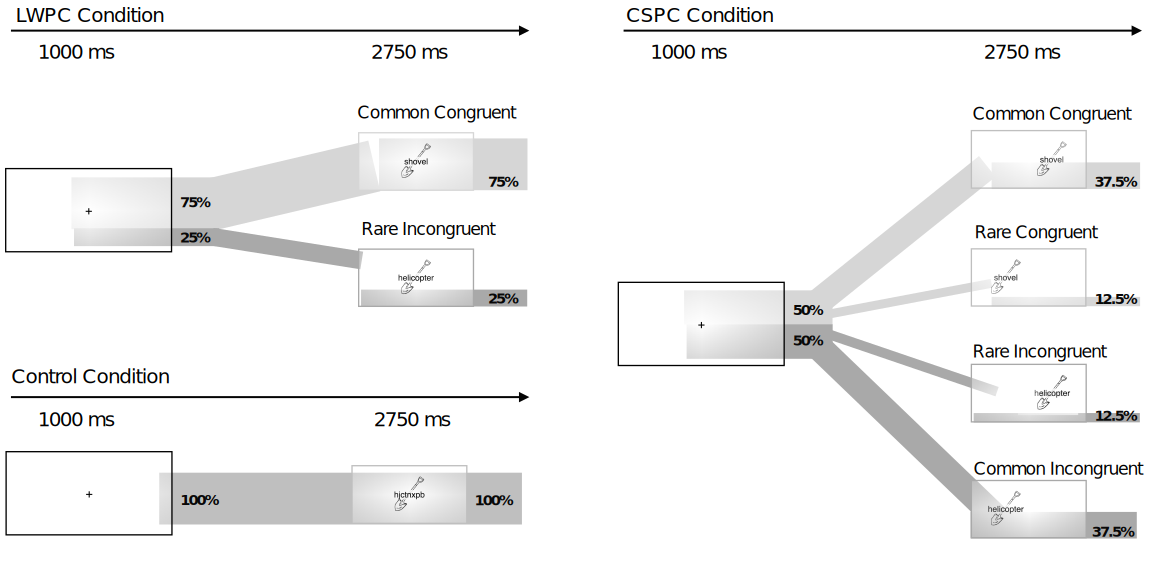
\includegraphics[width=\textwidth]{figure_1} \caption{Examples of the congruency and location proportions in a sample block, by condition. After a 1000 ms fixation cross and a 500 ms blank screen, a drawing and either a word (LWPC and CSPC conditions) or a random string of consonants (control condition) appeared. In the LWPC and the control condition, the drawing and words or letter strings always appeared in the center of the screen; in the CSPC condition they always appeared to the left or right of fixation. Note that in this example, the proportion of congruent trials in the LWPC condition block is 75\%, whereas in the CSPC condition that proportion is 50\%. However, in the CSPC condition the proportion congruency corresponded with the side of stimulus presentation, such that one side (in this example, the right side) was typically congruent (75\% of the time) and the other side (in this example, the left side) typically incongruent.}\label{fig:figure1}
\end{figure}



\hypertarget{analysis}{%
\subsection{Analysis}\label{analysis}}

\hypertarget{preprocessing}{%
\subsubsection{Preprocessing}\label{preprocessing}}

Analyses were conducted in R (R Core Team, 2021) using a variety of packages, including the R Tidyverse (Wickham et al., 2019) for data wrangling and graphing, tuneR for audio processing (Ligges, Krey, Mersmann, \& Schnackenberg, 2018), bayestestR (Makowski et al., 2021), CmdStanR (Gabry, Češnovar, \& Johnson, 2022), and tidybayes (Kay, 2021) for Bayesian analyses, and papaja (Aust \& Barth, 2021) for manuscript development. As expected, object naming accuracy was near ceiling in all conditions (mean accuracy = 99.6\%), and therefore response time (RT) was our only dependent variable. All the paper's results and deployed equations can be viewed in our open materials (\href{https://osf.io/z3tx7}{osf.io/z3tx7}), notably the RMarkdown (Allaire et al., 2022) document that generates the manuscript and results in-line.

Due to the high number of trials across participants (120 participants * 248 trials = 29,760), we leveraged the Google Cloud Speech API automatic speech transcriber in R (Edmondson, 2020, 2021) as a first pass for processing participants' verbal responses. Ziman, Heusser, Fitzpatrick, Field, and Manning (2018) previously validated this tool as a reliable transcriber of vocal responses from AMT psychological experiments. To guide the transcriber, it was fed a list of candidate words, which included the (most common) name of the image, of the overlaid label if it was an incongruent trial, and synonyms for the name of the image, since as Sz'ekely et al. (2003) showed these drawings can have numerous interpretations. Including these candidates increased their likelihood of being returned, but not enough to prohibit an unanticipated word from ever being transcribed.

After this first pass, we listened to the audio of, and manually transcribed, any trial whose automatic transcription did not match any of the candidate words. We corrected any unanticipated transcription that in fact was a correct response (923 trials), removed uninterpretable or seemingly nonsensical responses, and credited all unanticipated responses that were reasonable drawing interpretations (e.g., calling a dolphin a shark). We credited these responses liberally due to the fast pace of the task and the fact that the objects were partially occluded by the overlaid words or letter strings. Notably, analyzing only trials with the single most expected word response made no difference in any of the statistical tests. A list of the words credited as correct for each drawing is included in the data repository.

The first trial of each block was discarded from further analyses. We then removed any trial with at least one of the following features: it did not occur in full browser screen (0.1\% of trials); participants gave a blank (0.6\%) or nonsensical response (0.6\%); they had answered with the same response on a previous trial or that response had previously been a word label (1.3\%); the VoiceExperiment package (Nett, 2021) failed to detect a voice onset (2.5\%); a response occurred within 300 ms of stimulus onset (0.02\%) or after stimulus offset (0.8\%); or any additional trial preceded by any one of these pruned trials. This trimming procedure left 25,914 trials for the RT analysis (88.5\% of the 29,280 trials).

To process RTs, we used the ``onsets'' function from the R package VoiceExperiment (Nett, 2021). This function was built specifically for determining vocal RTs in psychological experiments, and it produced highly similar RTs to our manual evaluation of a sampling of responses, even for responses with filler words or sounds.

\hypertarget{statistical-models}{%
\subsubsection{Statistical Models}\label{statistical-models}}

We analyzed LWPC and CSPC effects using both a frequentist model and a set of competing Bayesian models. Most elements of the models were identical, and they produced equivalent results. The models regressed RT onto trial congruency and context congruency, and treated participants and specific drawings as random effects.

Note that because of the nature of the data collection, all RTs in this study were subject to a global delay of a few-hundred ms due to lag in the Internet's capture of user audio. This inflates raw RTs with some non-systematic lag that is constant within each block of trials, but can differ between blocks. To account for this, in the CSPC condition, whose congruency proportions were constant between blocks, we re-ran the frequentist generalized linear mixed model post-hoc with block as a nested random intercept; doing so did not change the results. The LWPC condition involves a between-block design, and we thus could not control for average block RT; however, given the random nature of the lag, its effect was expected to average out over conditions and participants. This was corroborated by the fact that we observed the expected LWPC effect (see the Results section). We also included block number as a crossed random intercept, and this addition did not change our results.

We employed an lme4 (Bates, Mächler, Bolker, \& Walker, 2015) frequentist model that used a BOBYQA optimizer to avoid convergence warnings, and assumed the RTs fit a gamma distribution, which has been shown to better capture a raw RT distribution than a normal distribution (Lo \& Andrews, 2015). For the brms (Bürkner, 2017, 2018, 2021) Bayesian analyses, we tested three RT distributions (ex-Gaussian, skew normal, and shifted lognormal) and three model formulas for a total of nine model fits per task (see Supplementary Table 1 for the competing models). Each model's priors reflected effect sizes reported in Spinelli et al. (2019) regarding the LWPC effect and in Bugg et al. (2020) regarding the CSPC effect. We ran 10,000 warm-up iterations and generated 10,000 posterior samples per parameter per model across four MCMC chains. Of the nine fits, this paper reports statistics from the one with the lowest leave-one-out information criterion (LOOIC) in both tasks, model 6 in Supplementary Table 1. That model assumes a shifted lognormal RT distribution and reads as follows in R syntax:

\[\begin{aligned}RT \sim Congruency * Bias + (Congruency + Bias | Participant)\\\text{+ } (Congruency + Bias | Participant)\\\text{+ } (Congruency + Bias | Unique Drawing)\\\text{+ } (1 | Unique Block \text{ or } Block Number)\end{aligned}\]

We corroborated that this Bayesian model converged via visual inspection of trace plots (see Supplementary Figures 1 and 2) and because \(\widehat{R}\) values ranged between 1.000 and 1.009, below the recognized 1.1 threshold (Gelman \& Rubin, 1992). We then evaluated the model's parameters using the full Region of Practical Equivalence (ROPE) (Makowski, Ben-Shachar, Chen, \& Lüdecke, 2019), the percentage of a coefficient's whole posterior within the null region. We defined the predetermined ROPE null region for each parameter as -.1 to .1 in log units. A coefficient is significant if its posterior overlaps with the full ROPE less than 5\%; it is considered null if it overlaps with the full ROPE more than 95\%; and any overlap between 5\% and 95\% is undetermined (Makowski et al., 2019).

Finally, we also ran a post-hoc Bayesian power analysis on the CSPC effect after the ROPE for 60 participants was undetermined (\(\upbeta\) = -3.3, \emph{SE} = 3.3, z = -0.99, \emph{p} = 0.322, ROPE = {[}-6.21 ms, 6.21 ms{]}, 69.56\% in ROPE, BF = 0.334; see the Results section). To reduce computational demand, the power analysis omitted previous trial RT, resulting in model 3 listed in Supplementary Table 1. We determined power as the number of full ROPE scores less than 5\% or greater than 95\% among 120 simulations each on 300 artificial participants.

\hypertarget{results}{%
\section{Results}\label{results}}

The two sets of results we report address, first, general congruency effects while taking into account baseline object naming RTs, and second, proportion-related modulation of congruency effects as a function of listwide or spatial context.

\hypertarget{congruency-effects}{%
\subsection{Congruency Effects}\label{congruency-effects}}

For general congruency effects, we used the control condition to subtract out image-specific baseline object naming times (under superimposed letters) from their respective congruent and incongruent RTs. Thus, we calculated baseline RTs for each image as the mean object-naming RT (over participants) for that image in the control condition, and then we calculated a difference-scored RT for each LWPC and CSPC group trial as that trial's RT minus its drawing's control-condition-derived baseline RT.

In order to establish whether congruent labels would facilitate and unrelated words interfere with object naming relative to baseline (control condition) naming times, we analyzed whether the average congruent trial difference-scored RT was significantly less than zero, which would indicate a facilitation effect (Rosinski, Golinkoff, \& Kukish, 1975). We then did the same for incongruent trials, where a score significantly greater than zero would indicate an interference effect. We used a generalized linear mixed-effects model from the lme4 package (Bates et al., 2015) that regressed difference-score RTs with random intercepts of participant ID and picture identity. As seen in Table 1 and Figure 2, we found clear evidence of a facilitation effect in congruent trials, and of an interference effect in the corresponding incongruent trials. Thus, we observed robust evidence for semantic facilitation and interference effects in this object-naming protocol.

\begin{table}[ht]
\centering
\caption{Frequentist generalized linear mixed-effects model estimates of a congruency
effect among each combination of condition, trial congruency, and typical
block (in LWPC condition) or location (in CSPC condition) congruency, using
difference-scored RTs} 
\begin{tabular}{lll|ccccc}
  \hline
Condition & Congruency & Bias & $\beta$ & \emph{SE} & \emph{t} & \emph{DF} & \emph{p} \\ 
  \hline
LWPC & Congruent & Mostly Congruent & -203.8 & 30.6 & -6.65 & 29.3 & $<$ .001 \\ 
  LWPC & Congruent & Mostly Incongruent & -145.1 & 33.2 & -4.37 & 25.8 & $<$ .001 \\ 
  LWPC & Incongruent & Mostly Congruent & 162.6 & 40.5 & 4.02 & 13 & .001 \\ 
  LWPC & Incongruent & Mostly Incongruent & 133.5 & 36.1 & 3.70 & 28.1 & $<$ .001 \\ 
  CSPC & Congruent & Mostly Congruent & -114.1 & 10.2 & -11.16 & 237.9 & $<$ .001 \\ 
  CSPC & Congruent & Mostly Incongruent & -117.1 & 10.8 & -10.84 & 237.3 & $<$ .001 \\ 
  CSPC & Incongruent & Mostly Congruent & 196.3 & 13.4 & 14.68 & 236.1 & $<$ .001 \\ 
  CSPC & Incongruent & Mostly Incongruent & 191 & 12 & 15.97 & 235.7 & $<$ .001 \\ 
   \hline
\end{tabular}
\end{table}

\begin{figure}[!h]
\includegraphics[width=\textwidth]{manuscript_files/figure-latex/figure2-1} \caption{Response time as a function of condition, trial congruency, and listwide (LWPC condition) or location-based (CSPC condition) proportion congruency. The vertical distributions chart every trial for every participant. Note that the y axis measures a given LWPC condition or CSPC condition RT relative to the baseline control RT for the corresponding drawing, such that numbers below zero represent facilitation and above zero represent interference effects. Asterisks to the left of their respective violin plot indicate a significant difference between congruent and incongruent RTs whereas asterisks to the right of their respective violin plot indicate a significant difference from zero.}\label{fig:figure2}
\end{figure}



\hypertarget{contextual-modulation-of-congruency-effects}{%
\subsection{Contextual Modulation of Congruency Effects}\label{contextual-modulation-of-congruency-effects}}

We next sought to assess adjustments in control as a function of listwide and spatial context manipulations of the proportion of congruent trials. To this end, we separately analyzed how the congruency of a trial interacted with the proportion of congruent trials as varied over blocks (LWPC condition) or between screen locations (CSPC condition). The results are listed in Table 2. We observed a clear LWPC effect: trial congruency interacted significantly with the block-wise proportion congruent factor (\(\upbeta\) = -93.5, \emph{SE} = 3.6, z = -26.27, \emph{p} \textless{} .001, ROPE = {[}-5.58 ms, 5.58 ms{]}, 0\% in ROPE, BF \textgreater{} 1000), as mean congruency effects were smaller in the context of mostly-incongruent blocks (mean = 252 ms) than in mostly-congruent blocks (mean = 349 ms). This was driven both by congruent trial RTs being significantly faster in mostly-congruent blocks compared to in mostly-incongruent ones (\(\upbeta\) = 56.1, \emph{SE} = 5.2, z = 10.83, \emph{p} \textless{} .001), as well as by incongruent trials being responded to significantly more quickly in mostly-incongruent than in mostly-congruent blocks (\(\upbeta\) = -39.0, \emph{SE} = 7.2, z = -5.42, \emph{p} \textless{} .001). Thus, we replicated the within-participant LWPC effect with trial-unique stimuli while controlling for picture-specific baseline naming times.

\begin{table}[!htbp] \centering    \caption{Raw RTs regressed in a frequentist generalized linear mixed-effects model over trial congruency, block- or location-wise congruency, and previous trial RT}    \label{}  \begin{tabular}{@{\extracolsep{5pt}}lD{.}{.}{-1} D{.}{.}{-1} }  \\[-1.8ex]\hline  \hline \\[-1.8ex]   & \multicolumn{2}{c}{Regression Coefficients of Raw Response Times} \\  \cline{2-3}  \\[-1.8ex] & \multicolumn{2}{c}{By condition} \\   & \multicolumn{1}{c}{LWPC} & \multicolumn{1}{c}{CSPC} \\  \hline \\[-1.8ex]   Trial congruency & 347.4^{***}$ $(3.6) & 294.3^{***}$ $(3.0) \\    Congruency bias (block or location) & 56.1^{***}$ $(3.2) & -2.8$ $(2.4) \\    Trial congruency X Congruency bias & -93.5^{***}$ $(3.6) & -3.3$ $(3.3) \\    Intercept & 1,162.4^{***}$ $(5.0) & 1,232.5^{***}$ $(3.2) \\   \hline \\[-1.8ex]  Observations & \multicolumn{1}{c}{6,453} & \multicolumn{1}{c}{13,053} \\  Log Likelihood & \multicolumn{1}{c}{-44,156.5} & \multicolumn{1}{c}{-89,330.0} \\  \hline  \hline \\[-1.8ex]  \textit{Note:}  & \multicolumn{2}{r}{$^{*}$p$<$0.05; $^{**}$p$<$0.01; $^{***}$p$<$0.001} \\  \end{tabular}  \end{table}

In contrast, we did not detect evidence for a CSPC effect in the condition where the proportion of congruent trials was manipulated as a function of stimulus location, as there was no interaction between trial congruency and location (\(\upbeta\) = -3.3, \emph{SE} = 3.3, z = -0.99, \emph{p} = 0.322, ROPE = {[}-6.21 ms, 6.21 ms{]}, 69.56\% in ROPE, BF = 0.334). Accordingly, neither the difference in congruent trial RTs between mostly-congruent and mostly-incongruent locations (\(\upbeta\) = -6.0, \emph{SE} = 3.3, z = -1.84, \emph{p} = 0.066), nor the difference in incongruent trial RTs between mostly-congruent and mostly-incongruent locations (\(\upbeta\) = -5.4, \emph{SE} = 4.5, z = -1.20, \emph{p} = 0.231) were significant. Post-hoc, we also explored whether a CSPC effect may have emerged only after participants had a block of experience to learn about the location-based proportion congruency; nevertheless, the results did not change when dropping the first block (interaction between trial congruency and location's typical congruency: \(\upbeta\) = 4.0, \emph{SE} = 7.8, z = 0.52, \emph{p} = 0.605)). Moreover, a post-hoc Bayesian power analysis indicated that a sample greater than 300 people would be required to detect or reject an effect with 0.80 power. This suggests that such an effect, if it did exist, would be so small as to arguably not to be of practical interest.

\hypertarget{discussion}{%
\section{Discussion}\label{discussion}}

In this study, we employed trial-unique stimuli in a picture-word interference task to probe whether one can obtain LWPC and/or CSPC effects in a within-participants design absent any episodic memory or baseline picture-naming time confounds. The results were clear-cut in that we observed very strong evidence for (baseline-corrected) interference and facilitation effects in the picture-word interference task, and for their modulation by the proportion of congruent trials when varied over blocks -- the LWPC effect. By contrast, we did not obtain any evidence for such modulation when the proportion of congruent trials was manipulated by spatial context rather than over time, that is, no CSPC effect could be detected. We discuss the implications of these two findings in turn.

Given the trial-unique nature of all target and distracter features in this study, the results of the LWPC manipulation provide unambiguous evidence for a control-based interpretation of listwide proportion congruent effects. Advancing on the study by Spinelli and colleagues (2019), the within-participant nature of our design makes the present findings directly comparable to the large majority of prior studies in this literature using non-unique stimuli, and the baseline picture-naming time correction rules out possible spurious effects of chance differences in naming difficulty in the assignment of stimuli to task conditions. Importantly, since the use of trial-unique stimuli preempts any effects of item-based or episodic control learning in the current study, these results provide strong evidence for a cumulative control-learning mechanism that operates at the level of task goals (i.e., ``name the pictures, ignore the words'') and is independent of the particulars of stimulus features presented on a given trial, as postulated by the conflict monitoring model and related theories (Botvinick et al. (2001), Jiang, Heller, and Egner (2014)).

Beyond providing particularly clean evidence for the existence of an LWPC effect in the absence of possible stimulus-response and episodic, item-based control learning effects, we hope that the current adaptation of Spinelli et al.'s (2019) protocol may also prove useful for future studies in methodological terms. First, at the technical level, the current data provide a proof-of-principle that vocal responding and automated response coding is feasible for use in online studies, thus opening up the possibility of fast and large-scale data acquisition with this task (for relevant code, see \url{github.com/jackdolgin/adaptive-control}). Second, at the conceptual level, the trial-unique picture-word interference protocol lends itself particularly well to addressing a crucial current question in the cognitive control literature, namely, what the interplay is between cumulative, task-goal adjustments in control based on recent control demand and the item-based, episodic reinstatement of control (e.g., Whitehead, Pfeuffer, and Egner (2020); Bugg and Egner (2021)). For instance, one could extend the current LWPC design to include a subset of trials where target stimuli reoccur, and gauge how the expected episodic reinstatement of control settings on these trials may interact with the current temporal context (low vs.~high proportion congruent block). A similar strategy has proven informative in the field of reward-guided decision making, where episodic cues have been found to sometimes override cumulative learning of the current context (Duncan, Doll, Daw, and Shohamy (2018)).

Turning to the CSPC manipulation, the current data add to the uncertainty over whether this phenomenon is reliable and does in fact reflect a pure association between location and control demands (Matthew J. C. Crump et al. (2017); Hutcheon and Spieler (2017); James R. Schmidt and Lemercier (2018); Bugg et al. (2020), Bugg and Egner (2021)). We found no evidence of a modulation of congruency effects by location, in spite of employing the same task and proportion bias as in the LWPC protocol, a large sample, and the horizontal axis for manipulating locations, which has been reported to be more potent than the vertical axis (Weidler, Pratt, and Bugg (2022)). Moreover, a post-hoc power analysis suggested that detecting a potential CSPC effect in the current protocol would require a sample of more than 300 participants. The latter observation indicates that a location-based CSPC effect for trial-unique items would be so weak that, even if it did existed, it would arguably be of little practical interest.

The lack of a CSPC effect in the current study could plausibly stem from the main factor that distinguishes this protocol from prior studies, namely, the use of trial-unique stimuli. The control-based interpretation of previous CSPC findings is that spatial locations (or other contextual features) become associated with particular control demands via an episodic binding process, and that presenting a stimulus in those locations would, reactively, retrieve or reinstate the associated control state (e.g., Matthew J. C. Crump and Milliken (2009)). The current findings suggest that for this type of episodic control to develop, there has to be at least some degree of stimulus recurrence in addition to the systematic linking between location and control demand. This was the case in previous demonstrations of the CSPC effect: using small stimulus sets, both the biased ``inducer'' items and unbiased ``transfer'' or ``diagnostic'' items were presented at the different locations many times over (e.g., Matthew J. C. Crump and Milliken (2009); Hutcheon and Spieler (2017); Matthew J. C. Crump et al. (2017); Bugg et al. (2020); Bugg and Egner (2021)). This may both make the location-demand association more easily apparent as well as perhaps making it more likely that participants (implicitly) consider employing episodic information for performing the task, which would clearly be discouraged in an environment of trial-unique stimuli, such as the present CSPC experiment. This speculative interpretation could be tested in future studies, but the key conclusion here is that location-demand association alone, absent any stimulus repetitions, does not appear to give rise to a CSPC effect.

In conclusion, using an optimized version of Spinelli et al.'s (2019) trial-unique picture-word interference protocol, we showed strong evidence for people adapting their attentional focus to time-varying control demands (the LWPC effect) without any target, distracter, or response recurrences, supportive of the existence of goal-based incremental control learning processes. By contrast, we did not obtain any evidence for such modulation when the proportion of congruent trials was manipulated by spatial context rather than over time, suggesting that the location-based CSPC effect requires some level of repeated episodic features beyond stimulus locations to emerge. These results provide new insights into the boundary conditions of how learning and memory processes guide cognitive control.

\newpage

\hypertarget{references}{%
\section{References}\label{references}}

\hypertarget{refs}{}
\begin{CSLReferences}{1}{0}
\leavevmode\vadjust pre{\hypertarget{ref-R-rmarkdown}{}}%
Allaire, J., Xie, Y., McPherson, J., Luraschi, J., Ushey, K., Atkins, A., \ldots{} Iannone, R. (2022). \emph{Rmarkdown: Dynamic documents for r}. Retrieved from \url{https://CRAN.R-project.org/package=rmarkdown}

\leavevmode\vadjust pre{\hypertarget{ref-js-annyang}{}}%
Ater, T. (2017). \emph{Annyang! Easily add speech recognition to your site}. Retrieved from \url{https://github.com/TalAter/annyang}

\leavevmode\vadjust pre{\hypertarget{ref-R-papaja}{}}%
Aust, F., \& Barth, M. (2021). \emph{Papaja: Prepare reproducible APA journal articles with r markdown}. Retrieved from \url{https://github.com/crsh/papaja}

\leavevmode\vadjust pre{\hypertarget{ref-lme42015}{}}%
Bates, D., Mächler, M., Bolker, B., \& Walker, S. (2015). Fitting linear mixed-effects models using {lme4}. \emph{Journal of Statistical Software}, \emph{67}(1), 1--48. \url{https://doi.org/10.18637/jss.v067.i01}

\leavevmode\vadjust pre{\hypertarget{ref-Botvinick_2001}{}}%
Botvinick, M. M., Braver, T. S., Barch, D. M., Carter, C. S., \& Cohen, J. D. (2001). Conflict monitoring and cognitive control. \emph{Psychological Review}, \emph{108}(3), 624--652. \url{https://doi.org/10.1037/0033-295x.108.3.624}

\leavevmode\vadjust pre{\hypertarget{ref-Braem_2019}{}}%
Braem, S., Bugg, J. M., Schmidt, J. R., Crump, M. J. C., Weissman, D. H., Notebaert, W., \& Egner, T. (2019). Measuring adaptive control in conflict tasks. \emph{Trends in Cognitive Sciences}, \emph{23}(9), 769--783. \url{https://doi.org/10.1016/j.tics.2019.07.002}

\leavevmode\vadjust pre{\hypertarget{ref-Bugg_2012}{}}%
Bugg, J. M., \& Crump, M. J. C. (2012). In support of a distinction between voluntary and stimulus-driven control: A review of the literature on proportion congruent effects. \emph{Frontiers in Psychology}, \emph{3}. \url{https://doi.org/10.3389/fpsyg.2012.00367}

\leavevmode\vadjust pre{\hypertarget{ref-Bugg_2021}{}}%
Bugg, J. M., \& Egner, T. (2021). The many faces of learning-guided cognitive control. \emph{Journal of Experimental Psychology: Learning, Memory, and Cognition}, \emph{47}(10), 1547--1549. \url{https://doi.org/10.1037/xlm0001075}

\leavevmode\vadjust pre{\hypertarget{ref-Bugg_2011}{}}%
Bugg, J. M., Jacoby, L. L., \& Chanani, S. (2011). Why it is too early to lose control in accounts of item-specific proportion congruency effects. \emph{Journal of Experimental Psychology: Human Perception and Performance}, \emph{37}(3), 844--859. \url{https://doi.org/10.1037/a0019957}

\leavevmode\vadjust pre{\hypertarget{ref-Bugg_2020}{}}%
Bugg, J. M., Suh, J., Colvett, J. S., \& Lehmann, S. G. (2020). What can be learned in a context-specific proportion congruence paradigm? Implications for reproducibility. \emph{Journal of Experimental Psychology: Human Perception and Performance}, \emph{46}(9), 1029--1050. \url{https://doi.org/10.1037/xhp0000801}

\leavevmode\vadjust pre{\hypertarget{ref-brms2017}{}}%
Bürkner, P.-C. (2017). {brms}: An {R} package for {Bayesian} multilevel models using {Stan}. \emph{Journal of Statistical Software}, \emph{80}(1), 1--28. \url{https://doi.org/10.18637/jss.v080.i01}

\leavevmode\vadjust pre{\hypertarget{ref-brms2018}{}}%
Bürkner, P.-C. (2018). Advanced {Bayesian} multilevel modeling with the {R} package {brms}. \emph{The R Journal}, \emph{10}(1), 395--411. \url{https://doi.org/10.32614/RJ-2018-017}

\leavevmode\vadjust pre{\hypertarget{ref-R-brms}{}}%
Bürkner, P.-C. (2021). \emph{Brms: Bayesian regression models using stan}. Retrieved from \url{https://CRAN.R-project.org/package=brms}

\leavevmode\vadjust pre{\hypertarget{ref-Chiu_2019}{}}%
Chiu, Y.-C., \& Egner, T. (2019). Cortical and subcortical contributions to context-control learning. \emph{Neuroscience \&Amp; Biobehavioral Reviews}, \emph{99}, 33--41. \url{https://doi.org/10.1016/j.neubiorev.2019.01.019}

\leavevmode\vadjust pre{\hypertarget{ref-Crump_2017}{}}%
Crump, Matthew J. C., Brosowsky, N. P., \& Milliken, B. (2017). Reproducing the location-based context-specific proportion congruent effect for frequency unbiased items: A reply to hutcheon and spieler (2016). \emph{Quarterly Journal of Experimental Psychology}, \emph{70}(9), 1792--1807. \url{https://doi.org/10.1080/17470218.2016.1206130}

\leavevmode\vadjust pre{\hypertarget{ref-Crump_2006}{}}%
Crump, Matthew J. C., Gong, Z., \& Milliken, B. (2006). The context-specific proportion congruent stroop effect: Location as a contextual cue. \emph{Psychonomic Bulletin \&Amp; Review}, \emph{13}(2), 316--321. \url{https://doi.org/10.3758/bf03193850}

\leavevmode\vadjust pre{\hypertarget{ref-Crump_2009}{}}%
Crump, Matthew J. C., \& Milliken, B. (2009). Short article: The flexibility of context-specific control: Evidence for context-driven generalization of item-specific control settings. \emph{Quarterly Journal of Experimental Psychology}, \emph{62}(8), 1523--1532. \url{https://doi.org/10.1080/17470210902752096}

\leavevmode\vadjust pre{\hypertarget{ref-Duncan_2018}{}}%
Duncan, K., Doll, B. B., Daw, N. D., \& Shohamy, D. (2018). More than the sum of its parts: A role for the hippocampus in configural reinforcement learning. \emph{Neuron}, \emph{98}(3), 645--657.e6. \url{https://doi.org/10.1016/j.neuron.2018.03.042}

\leavevmode\vadjust pre{\hypertarget{ref-R-googleLanguageR}{}}%
Edmondson, M. (2020). \emph{googleLanguageR: Call google's natural language API, cloud translation API, cloud speech API and cloud text-to-speech API}. Retrieved from \url{https://CRAN.R-project.org/package=googleLanguageR}

\leavevmode\vadjust pre{\hypertarget{ref-R-googleCloudStorageR}{}}%
Edmondson, M. (2021). \emph{googleCloudStorageR: Interface with google cloud storage API}. Retrieved from \url{https://code.markedmondson.me/googleCloudStorageR/}

\leavevmode\vadjust pre{\hypertarget{ref-Egner_2017}{}}%
Egner, T. (2017). Conflict adaptation: Past, present, and future of the congruency sequence effect as an index of cognitive control. Wiley. \url{https://doi.org/10.1002/9781118920497.ch4}

\leavevmode\vadjust pre{\hypertarget{ref-Fraisse_1968}{}}%
Fraisse, P. (1968). Motor and verbal reaction times to words and drawings. \emph{Psychonomic Science}, \emph{12}(6), 235--236. \url{https://doi.org/10.3758/bf03331287}

\leavevmode\vadjust pre{\hypertarget{ref-R-cmdstanr}{}}%
Gabry, J., Češnovar, R., \& Johnson, A. (2022). \emph{Cmdstanr: R interface to CmdStan}.

\leavevmode\vadjust pre{\hypertarget{ref-Gelman_1992}{}}%
Gelman, A., \& Rubin, D. B. (1992). Inference from iterative simulation using multiple sequences. \emph{Statistical Science}, \emph{7}(4). \url{https://doi.org/10.1214/ss/1177011136}

\leavevmode\vadjust pre{\hypertarget{ref-H_bner_2016}{}}%
Hübner, R., \& Mishra, S. (2016). Location-specific attentional control is also possible in the simon task. \emph{Psychonomic Bulletin \&Amp; Review}, \emph{23}(6), 1867--1872. \url{https://doi.org/10.3758/s13423-016-1057-y}

\leavevmode\vadjust pre{\hypertarget{ref-Hutcheon_2017}{}}%
Hutcheon, T. G., \& Spieler, D. H. (2017). Limits on the generalizability of context-driven control. \emph{Quarterly Journal of Experimental Psychology}, \emph{70}(7), 1292--1304. \url{https://doi.org/10.1080/17470218.2016.1182193}

\leavevmode\vadjust pre{\hypertarget{ref-Jacoby_2003}{}}%
Jacoby, L. L., Lindsay, D. S., \& Hessels, S. (2003). Item-specific control of automatic processes: Stroop process dissociations. \emph{Psychonomic Bulletin \&Amp; Review}, \emph{10}(3), 638--644. \url{https://doi.org/10.3758/bf03196526}

\leavevmode\vadjust pre{\hypertarget{ref-Jiang_2014}{}}%
Jiang, J., Heller, K., \& Egner, T. (2014). Bayesian modeling of flexible cognitive control. \emph{Neuroscience \&Amp; Biobehavioral Reviews}, \emph{46}, 30--43. \url{https://doi.org/10.1016/j.neubiorev.2014.06.001}

\leavevmode\vadjust pre{\hypertarget{ref-R-tidybayes}{}}%
Kay, M. (2021). \emph{Tidybayes: Tidy data and geoms for bayesian models}. Retrieved from \url{https://CRAN.R-project.org/package=tidybayes}

\leavevmode\vadjust pre{\hypertarget{ref-King_2012}{}}%
King, J. A., Korb, F. M., \& Egner, T. (2012). Priming of control: Implicit contextual cuing of top-down attentional set. \emph{Journal of Neuroscience}, \emph{32}(24), 8192--8200. \url{https://doi.org/10.1523/jneurosci.0934-12.2012}

\leavevmode\vadjust pre{\hypertarget{ref-tuneR2018}{}}%
Ligges, U., Krey, S., Mersmann, O., \& Schnackenberg, S. (2018). \emph{{tuneR}: Analysis of music and speech}. Retrieved from \url{https://CRAN.R-project.org/package=tuneR}

\leavevmode\vadjust pre{\hypertarget{ref-Lo_2015}{}}%
Lo, S., \& Andrews, S. (2015). To transform or not to transform: Using generalized linear mixed models to analyse reaction time data. \emph{Frontiers in Psychology}, \emph{6}. \url{https://doi.org/10.3389/fpsyg.2015.01171}

\leavevmode\vadjust pre{\hypertarget{ref-Logan_1979}{}}%
Logan, G. D., \& Zbrodoff, N. J. (1979). When it helps to be misled: Facilitative effects of increasing the frequency of conflicting stimuli in a stroop-like task. \emph{Memory \&Amp; Cognition}, \emph{7}(3), 166--174. \url{https://doi.org/10.3758/bf03197535}

\leavevmode\vadjust pre{\hypertarget{ref-Lupker_1979}{}}%
Lupker, S. J. (1979). The semantic nature of response competition in the picture-word interference task. \emph{Memory \&Amp; Cognition}, \emph{7}(6), 485--495. \url{https://doi.org/10.3758/bf03198265}

\leavevmode\vadjust pre{\hypertarget{ref-MacLeod_1991}{}}%
MacLeod, C. M. (1991). Half a century of research on the stroop effect: An integrative review. \emph{Psychological Bulletin}, \emph{109}(2), 163--203. \url{https://doi.org/10.1037/0033-2909.109.2.163}

\leavevmode\vadjust pre{\hypertarget{ref-Makowski_2019}{}}%
Makowski, D., Ben-Shachar, M. S., Chen, S. H. A., \& Lüdecke, D. (2019). Indices of effect existence and significance in the bayesian framework. \emph{Frontiers in Psychology}, \emph{10}. \url{https://doi.org/10.3389/fpsyg.2019.02767}

\leavevmode\vadjust pre{\hypertarget{ref-R-bayestestR}{}}%
Makowski, D., Lüdecke, D., Ben-Shachar, M. S., Patil, I., Wilson, M. D., \& Wiernik, B. M. (2021). \emph{bayestestR: Understand and describe bayesian models and posterior distributions}. Retrieved from \url{https://easystats.github.io/bayestestR/}

\leavevmode\vadjust pre{\hypertarget{ref-Miller_2001}{}}%
Miller, E. K., \& Cohen, J. D. (2001). An integrative theory of prefrontal cortex function. \emph{Annual Review of Neuroscience}, \emph{24}(1), 167--202. \url{https://doi.org/10.1146/annurev.neuro.24.1.167}

\leavevmode\vadjust pre{\hypertarget{ref-R-VoiceExperiment}{}}%
Nett, T. (2021). \emph{VoiceExperiment: Analysis of vocal responses to psychological experiments}.

\leavevmode\vadjust pre{\hypertarget{ref-R-base}{}}%
R Core Team. (2021). \emph{R: A language and environment for statistical computing}. Vienna, Austria: R Foundation for Statistical Computing. Retrieved from \url{https://www.R-project.org/}

\leavevmode\vadjust pre{\hypertarget{ref-Rosinski_1975}{}}%
Rosinski, R. R., Golinkoff, R. M., \& Kukish, K. S. (1975). Automatic semantic processing in a picture-word interference task. \emph{Child Development}, \emph{46}(1), 247. \url{https://doi.org/10.2307/1128859}

\leavevmode\vadjust pre{\hypertarget{ref-Schmidt_2013}{}}%
Schmidt, James R. (2013). Questioning conflict adaptation: Proportion congruent and gratton effects reconsidered. \emph{Psychonomic Bulletin \&Amp; Review}, \emph{20}(4), 615--630. \url{https://doi.org/10.3758/s13423-012-0373-0}

\leavevmode\vadjust pre{\hypertarget{ref-Schmidt_2018_1}{}}%
Schmidt, James R. (2018). Evidence against conflict monitoring and adaptation: An updated review. \emph{Psychonomic Bulletin \&Amp; Review}, \emph{26}(3), 753--771. \url{https://doi.org/10.3758/s13423-018-1520-z}

\leavevmode\vadjust pre{\hypertarget{ref-Schmidt_2018}{}}%
Schmidt, James R., \& Lemercier, C. (2018). Context-specific proportion congruent effects: Compound-cue contingency learning in disguise. \emph{Quarterly Journal of Experimental Psychology}, \emph{72}(5), 1119--1130. \url{https://doi.org/10.1177/1747021818787155}

\leavevmode\vadjust pre{\hypertarget{ref-Spinelli_2019}{}}%
Spinelli, G., Perry, J. R., \& Lupker, S. J. (2019). Adaptation to conflict frequency without contingency and temporal learning: Evidence from the picture--word interference task. \emph{Journal of Experimental Psychology: Human Perception and Performance}, \emph{45}(8), 995--1014. \url{https://doi.org/10.1037/xhp0000656}

\leavevmode\vadjust pre{\hypertarget{ref-Starreveld_2016}{}}%
Starreveld, P. A., \& La Heij, W. (2016). Picture-word interference is a stroop effect: A theoretical analysis and new empirical findings. \emph{Psychonomic Bulletin \&Amp; Review}, \emph{24}(3), 721--733. \url{https://doi.org/10.3758/s13423-016-1167-6}

\leavevmode\vadjust pre{\hypertarget{ref-Stroop_1935}{}}%
Stroop, J. R. (1935). Studies of interference in serial verbal reactions. \emph{Journal of Experimental Psychology}, \emph{18}(6), 643--662. \url{https://doi.org/10.1037/h0054651}

\leavevmode\vadjust pre{\hypertarget{ref-Szekely_2003}{}}%
Sz'ekely, A., D'Amico, S., Devescovi, A., Federmeier, K., Herron, D., Iyer, G., \ldots{} Bates, E. (2003). Timed picture naming: Extended norms and validation against previous studies. \emph{Behavior Research Methods, Instruments, \&Amp; Computers}, \emph{35}(4), 621--633. \url{https://doi.org/10.3758/bf03195542}

\leavevmode\vadjust pre{\hypertarget{ref-Szekely_2004}{}}%
Szekely, A., Jacobsen, T., D'Amico, S., Devescovi, A., Andonova, E., Herron, D., \ldots{} Bates, E. (2004). A new on-line resource for psycholinguistic studies. \emph{Journal of Memory and Language}, \emph{51}(2), 247--250. \url{https://doi.org/10.1016/j.jml.2004.03.002}

\leavevmode\vadjust pre{\hypertarget{ref-Weidler_2022}{}}%
Weidler, B. J., Pratt, J., \& Bugg, J. M. (2022). How is location defined? Implications for learning and transfer of location-specific control. \emph{Journal of Experimental Psychology: Human Perception and Performance}, \emph{48}(4), 312--330. \url{https://doi.org/10.1037/xhp0000989}

\leavevmode\vadjust pre{\hypertarget{ref-Whitehead_2020}{}}%
Whitehead, P. S., Pfeuffer, C. U., \& Egner, T. (2020). Memories of control: One-shot episodic learning of item-specific stimulus-control associations. \emph{Cognition}, \emph{199}, 104220. \url{https://doi.org/10.1016/j.cognition.2020.104220}

\leavevmode\vadjust pre{\hypertarget{ref-tidyverse2019}{}}%
Wickham, H., Averick, M., Bryan, J., Chang, W., McGowan, L. D., François, R., \ldots{} Yutani, H. (2019). Welcome to the {tidyverse}. \emph{Journal of Open Source Software}, \emph{4}(43), 1686. \url{https://doi.org/10.21105/joss.01686}

\leavevmode\vadjust pre{\hypertarget{ref-Ziman_2018}{}}%
Ziman, K., Heusser, A. C., Fitzpatrick, P. C., Field, C. E., \& Manning, J. R. (2018). Is automatic speech-to-text transcription ready for use in psychological experiments? \emph{Behavior Research Methods}, \emph{50}(6), 2597--2605. \url{https://doi.org/10.3758/s13428-018-1037-4}

\end{CSLReferences}

\newpage

\setcounter{table}{0}
\renewcommand{\tablename}{Supplementary Table}
\setcounter{figure}{0}
\renewcommand{\figurename}{Supplementary Figure}

\begin{table}[ht]
\centering
\caption{Competing Bayesian model specifications for analyzing response times. Each row
corresponds to one of nine model variants, defined by a combination of (a) the
assumed RT distribution (Ex-Gaussian, skew-normal, or shifted lognormal) and
(b) the fixed and random effects included in the regression formula. The final
column indicates whether random intercepts, random slopes, or both were modeled
for the participant and item factors (and, where relevant, the block factor).} 
\begin{tabular}{ll|p{4in}}
 Model & Family & Random Effects \\ 
  \hline
1 & Ex-Gaussian & (1 $|$ Participant) + (1 $|$ Unique Drawing) + (1 $|$ Unique Block or Block Number) \\ 
   \hline
2 & Skew Normal & (1 $|$ Participant) + (1 $|$ Unique Drawing) + (1 $|$ Unique Block or Block Number) \\ 
   \hline
3 & Shifted Lognormal & (1 $|$ Participant) + (1 $|$ Unique Drawing) + (1 $|$ Unique Block or Block Number) \\ 
   \hline
4 & Ex-Gaussian & (Congruency + Bias $|$ Participant) + (Congruency + Bias $|$ Participant) + (Congruency + Bias $|$ Unique Drawing) + (1 $|$ Unique Block or Block Number) \\ 
   \hline
5 & Skew Normal & (Congruency + Bias $|$ Participant) + (Congruency + Bias $|$ Participant) + (Congruency + Bias $|$ Unique Drawing) + (1 $|$ Unique Block or Block Number) \\ 
   \hline
6 & Shifted Lognormal & (Congruency + Bias $|$ Participant) + (Congruency + Bias $|$ Participant) + (Congruency + Bias $|$ Unique Drawing) + (1 $|$ Unique Block or Block Number) \\ 
   \hline
7 & Ex-Gaussian & (Congruency $|$ Participant) + (1 $|$ Unique Drawing) + (1 $|$ Unique Block or Block Number) \\ 
   \hline
8 & Skew Normal & (Congruency $|$ Participant) + (1 $|$ Unique Drawing) + (1 $|$ Unique Block or Block Number) \\ 
   \hline
9 & Shifted Lognormal & (Congruency $|$ Participant) + (1 $|$ Unique Drawing) + (1 $|$ Unique Block or Block Number) \\ 
   \hline
\end{tabular}
\end{table}

\begin{figure}[!h]
\includegraphics[width=\textwidth]{manuscript_files/figure-latex/suppfig1-1} \caption{Trace plots for each parameter in the best-fitting Bayesian model for the LWPC data (shifted-lognormal distribution). Each panel displays draws over MCMC iterations for one parameter, with four chains overlaid. The close overlap among chains and lack of trending indicate good convergence.}\label{fig:suppfig1}
\end{figure}

\begin{figure}[!h]
\includegraphics[width=\textwidth]{manuscript_files/figure-latex/suppfig2-1} \caption{Trace plots for each parameter in the best-fitting Bayesian model for the CSPC data (shifted-lognormal distribution). Each panel shows MCMC samples for one parameter, with four chains overlaid. As with Figure 1, the chain traces suggest stable estimates and satisfactory mixing.}\label{fig:suppfig2}
\end{figure}


\end{document}
